
\documentclass[12pt]{article}
\usepackage[utf8]{inputenc}
\usepackage[T1]{fontenc}
\usepackage{amsmath}
\usepackage{physics}

\usepackage{amsfonts}
\usepackage{amssymb}
\usepackage[version=4]{mhchem}
\usepackage{stmaryrd}

\usepackage{listings} % Required for insertion of code
\usepackage{xcolor} % Required for custom colors
\usepackage{graphicx}

% Define custom colors
\definecolor{codegreen}{rgb}{0,0.6,0}
\definecolor{codegray}{rgb}{0.5,0.5,0.5}
\definecolor{codepurple}{rgb}{0.58,0,0.82}
\definecolor{backcolour}{rgb}{0.95,0.95,0.92}

% Setup the style for code listings
\lstdefinestyle{mystyle}{
    backgroundcolor=\color{backcolour},   
    commentstyle=\color{codegreen},
    keywordstyle=\color{magenta},
    numberstyle=\tiny\color{codegray},
    stringstyle=\color{codepurple},
    basicstyle=\ttfamily\footnotesize,
    breakatwhitespace=false,         
    breaklines=true,                 
    captionpos=b,                    
    keepspaces=true,                 
    numbers=left,                    
    numbersep=5pt,                  
    showspaces=false,                
    showstringspaces=false,
    showtabs=false,                  
    tabsize=2
}

% Activate the style
\lstset{style=mystyle}


\begin{document}
READING: Section 19.1-19.3 in Shankar on scattering and the Born approximation. PROBLEMS:
\section{}
\begin{enumerate}
  \setcounter{enumi}{20}
  \item Demonstrate our claim in the long solenoid discussion that the solution to the Schrödinger equation when there is a flux $\Phi$ in the solenoid is:
\end{enumerate}

$$
\psi(\mathbf{x}, t)=\psi_{L}(\mathbf{x}, t) e^{i q g_{L}(\mathbf{x})}+\psi_{R}(\mathbf{x}, t) e^{i q g_{R}(\mathbf{x})}
$$

where

$$
\begin{array}{ll}
g_{L}(\mathbf{x}) \equiv \int_{\mathbf{x}_{0}}^{\mathbf{x}} d \mathbf{x}^{\prime} \cdot \mathbf{A}(\mathbf{x}) & \text { along a left path } \\
g_{R}(\mathbf{x}) \equiv \int_{\mathbf{x}_{0}}^{\mathbf{x}} d \mathbf{x}^{\prime} \cdot \mathbf{A}(\mathbf{x}) & \text { along a right path }
\end{array}
$$

and $\psi_{L, R}(\mathbf{x}, t)$ satisfy the Schrödinger equation when $\Phi=0$.
\subsection{}
In case the Hamiltonian we wanted to solve was:
\begin{equation}
  H=\frac{1}{2 m}[\mathbf{p}-q \mathbf{A}(\mathbf{x}, t)]^{2}
\end{equation}
Substituting the form for the momentum operator, this becomes:
\begin{equation}
  H=\frac{1}{2 m}[-i \nabla -q \mathbf{A}(\mathbf{x}, t)]^{2}
\end{equation}
We want to show that the Schrödinger equation satisfies this relation for the left and right sides independently.
We are given:
\begin{equation}
  \Psi  = \Phi_L + \Phi_R 
\end{equation}
Where:
\begin{equation}
  \Phi_L = \psi_{L}(\mathbf{x}, t) e^{i q g_{L}(\mathbf{x})}
\end{equation}
We are really only interested in proving for the left side, and then the right side follows by symmetry, and then we can just use the superposition principle to get that the total wave function satisfies the Schrödinger equation.
Operating the form for the Hamiltonian on $\Phi_L$:
\begin{equation}
  H \Phi_L = \frac{1}{2 m}[-i \nabla -q \mathbf{A}(\mathbf{x}, t)]^{2} \Phi_L
\end{equation}
Let us consider the expansion of the inside of the parentheses:
\begin{equation}
  \left[-i \nabla -q \mathbf{A}(\mathbf{x}, t)\right]^{2} = \left[-i \nabla -q \mathbf{A}(\mathbf{x}, t)\right] \left[-i \nabla -q \mathbf{A}(\mathbf{x}, t)\right] = - \nabla^2 + i q \nabla \cdot \mathbf{A} + i q \mathbf{A} \cdot \nabla + q^2 \mathbf{A}^2
\end{equation}
Let us consider the effects of various of these terms on our wave function:
\begin{equation}
  \nabla \Phi_L = \nabla \psi_{L}(\mathbf{x}, t) e^{i q g_{L}(\mathbf{x})} + \psi_{L}(\mathbf{x}, t) e^{i q g_{L}(\mathbf{x})} \times i q \times \nabla g_{L}(\mathbf{x})
\end{equation}
Now let us consider the action of the nabla operator on $g_L$. Along the left path, this is just the vector potential for that path:
\begin{equation}
  \nabla g_L(\mathbf{x}) = \mathbf{A}_L(\mathbf{x})
\end{equation}
because
\begin{equation}
  g_L(\mathbf{x}) - g_L() = \int_{\mathbf{x}_0}^{\mathbf{x}} d \mathbf{x} \cdot \mathbf{A}_L(\mathbf{x})
\end{equation}
We can choose a gauge such that the vector potential has $\nabla \cdot \mathbf{A} = 0$. We do this by letting $\mathbf{A} \rightarrow \mathbf{A} + \nabla \chi$ where we have $\nabla^2 \chi = -\nabla \cdot \mathbf{A}$. With this, we can have:
\begin{equation}
  \nabla \cdot (\Phi_L \mathbf{A}) = \nabla \Phi_L \cdot \mathbf{A} + \Phi_L \nabla \cdot \mathbf{A} = \nabla \Phi_L \cdot \mathbf{A}
\end{equation}
We also can consider the relation of $\nabla^2$ operating on $\Phi _L$:
\begin{equation}
\begin{aligned}
  \nabla^2 \Psi_L e^{i q g_L(\mathbf{x})} &= \nabla(\nabla \psi_{L}(\mathbf{x}, t) e^{i q g_{L}(\mathbf{x})} + iq\psi_{L}(\mathbf{x}, t) e^{i q g_{L}(\mathbf{x})} \nabla g_{L}(\mathbf{x}))\\
\end{aligned}
\end{equation}
In an effort to simplify notation, we will have $\psi  \equiv \psi_L $ and $\alpha \equiv i q g_L(\mathbf{x})$.
Just rewriting what we previously found:
\begin{equation}
  \nabla^2 \psi e^{\alpha} = \nabla(\nabla \psi e^{\alpha} + \psi \nabla e^{\alpha}) = \nabla^2 \psi e^{\alpha} + 2 \nabla\psi \nabla\alpha e^{\alpha} + \psi (\nabla^2 \alpha e^{\alpha} + \nabla \alpha \nabla \alpha e^{\alpha}) 
\end{equation}
Factoring out the exponential term that is present in every peace, we get:
\begin{equation}
  = e^{\alpha} \left( \nabla^2 \psi + 2 \nabla \psi \nabla \alpha + \psi \nabla^2 \alpha + \psi \nabla \alpha \nabla \alpha \right)
\end{equation}
The third term is given by:
\begin{equation}
  \nabla^2 \alpha = \nabla^2 (i q g_L(\mathbf{x})) = i q \nabla \cdot \nabla g_L(\mathbf{x}) = i q \nabla \cdot \mathbf{A}_L(\mathbf{x}) = 0
\end{equation}
So we are left with:
\begin{equation}
  \nabla^2 \psi e^{\alpha} = e^{\alpha} \left( \nabla^2 \psi + 2 \nabla \psi \nabla \alpha + \psi \nabla \alpha \nabla \alpha \right)
\end{equation}
We can now consider the action of the Hamiltonian on $\Phi_L$:
\begin{equation}
    H \Phi_L = \cdots
\end{equation}
I was working with a friend while he was doing this, but I am not quite following the algebra from his solution. I do know that he eventually was able to get to the result:
\begin{equation}
  H \Phi_L = -\frac{e^{\alpha}}{2m} \nabla^2 \psi = e^{\alpha} \left( H \psi \right)
\end{equation}
Now, we can use the assertion for the time-dependent Schrödinger equation:
\begin{equation}
  = e^{\alpha} i \partial_t \psi 
\end{equation}
We want to bring the complex exponential inside of the parenthesis, but we have to flip the sign:
\begin{equation}
  = -i \partial_t \psi e^{\alpha}
\end{equation}
So we have shown that this left-side solution satisfies the Schrödinger equation when in the Coulomb gauge. The same process can be done with the right-side solution. And then when we superimpose the two, the sum $\Phi_L + \Phi_R$ will also satisfy the Schrödinger equation.
\begin{enumerate}
  \setcounter{enumi}{21}
  \item Prove the theorem (essentially exercise 18.4.4 in text):
\end{enumerate}
\section{}
Theorem: Let the Hamiltonian for a charged particle interacting with an electromagnetic field be $H$ :

$$
H=\frac{1}{2 m}[\mathbf{p}-q \mathbf{A}(\mathbf{x}, t)]^{2}+q \Phi(\mathbf{x}, t)+U(\mathbf{x}, t)
$$

Let $H^{\prime}$ be the Hamiltonian obtained from $H$ by a gauge transformation:

$$
\begin{aligned}
\mathbf{A}(\mathbf{x}, t) & \rightarrow \mathbf{A}^{\prime}(\mathbf{x}, t)=\mathbf{A}(\mathbf{x}, t)+\nabla \chi(\mathbf{x}, t) \\
\Phi(\mathbf{x}, t) & \rightarrow \Phi^{\prime}(\mathbf{x}, t)=\Phi(\mathbf{x}, t)-\partial_{t} \chi(\mathbf{x}, t)
\end{aligned}
$$
If $i \partial_{t} \psi=H \psi$ and $i \partial_{t} \psi^{\prime}=H^{\prime} \psi^{\prime}$, then

$$
\psi^{\prime}(\mathbf{x}, t)=e^{i q \chi(\mathbf{x}, t)} \psi(\mathbf{x}, t)
$$
We will start by making the ansatz that $\Psi^{\prime} = e^{i q \chi(\mathbf{x}, t)} \Psi$.
We will call the first time dependent short ensure equation, $A$, and the second, $B$.
and if we have guessed $\Psi^{\prime}$ correctly, then $B$ is true. 
We want to consider the relationship:
\begin{equation}
  e^{-i q \chi(\mathbf{x}, t)} B - A
\end{equation}

\subsection{}
The hambletonian with the gauge transformation is given by the same, but with the prime notation:
\begin{equation}
  H^{\prime}=\frac{1}{2 m}[\mathbf{p}-q \mathbf{A}^{\prime}(\mathbf{x}, t)]^{2}+q \Phi^{\prime}(\mathbf{x}, t)+U(\mathbf{x}, t)
\end{equation}
Plugging in the relations for the crimes:
\begin{equation}
  H^{\prime}=\frac{1}{2 m}[\mathbf{p}-q \mathbf{A}(\mathbf{x}, t) - q \nabla \chi(\mathbf{x}, t)]^{2}+q \Phi(\mathbf{x}, t) - q \partial_{t} \chi(\mathbf{x}, t) + U(\mathbf{x}, t)
\end{equation}
We assume that our solution is like $e^{i q \chi(\mathbf{x}, t)} \psi(\mathbf{x}, t)$, so we can plug this in to the Hamiltonian:

\section{}
\begin{enumerate}
  \setcounter{enumi}{22}
  \item Exercise 18.5.2 in the text, on the photoelectric effect.
\subsection{}
Actually, we have:
\begin{equation}
  \sigma =\frac{128 a_0^3 \pi e^2 p_f^3}{3 m \hbar^3 \omega c\left[1+p_f^2 a_0^2 / \hbar^2\right]^4}
\end{equation}
We aval with this to:
\begin{equation}
  \sigma = 1.31204968079106 \cdot 10^{-34} m^2
\end{equation}
% Inline Python code in the document
\begin{lstlisting}[language=Python]
from sympy import symbols, sqrt, pi, latex

# Constants
eV_to_J = 1.602e-19  # Conversion from eV to Joules
Ry_to_eV = 13.6  # Conversion from Rydbergs to eV
a_0 = 0.529e-10  # Bohr radius in meters
m = 9.11e-31  # Electron mass in kg
e = 1.6e-19  # Elementary charge in Coulombs
c = 3e8  # Speed of light in m/s
hbar = 1.054e-34  # Reduced Planck's constant in Js

# Kinetic energy in Rydbergs
KE_Ry = 10
# Convert Ry to eV to J
KE_J = KE_Ry * Ry_to_eV * eV_to_J

# Calculate the momentum p_f using the relation E = p^2/2m (non-relativistic kinetic energy)
# p_f = sqrt(2*m*E)
p_f_value = sqrt(2 * m * KE_J)


# Calculate the second expression
omega = (KE_Ry * Ry_to_eV * eV_to_J) / hbar  # Angular frequency
second_expression = (128 * a_0**3 * pi * e**2 * p_f_value**3) / (3 * m * hbar**3 * omega * c * (1 + p_f_value**2 * a_0**2 / hbar**2)**4)

# Print the second result in LaTeX
print(latex(second_expression.evalf()))
\end{lstlisting}
That of the atom is much smaller:
% Inline Python code in the document
\begin{lstlisting}[language=Python]
# compute the atoms geometric cross section comma which is given by a_0^2\pi
pi = 3.14159265358979323846
atoms_cross_section = a_0**2 * pi
print(latex(atoms_cross_section))
\end{lstlisting}
\begin{equation}
  \sigma_{\text{atom}} = 8.79146429773221 \cdot 10^{-21} m^2
\end{equation}
\subsection{}
The 1s orbital is spherically symmetric and its bohr radius has an inverse dependence on the charge of the atom $Z$. Working under the assumption given in the problem that $\frac{p_fa_0}{\hbar} \gg 1$, the formula for the case section becomes:
\begin{equation}
  \sigma = \frac{128 a_0^3 \pi e^2 p_f^3}{3 m \hbar^3 \omega c(p_f^2 a_0^2 / \hbar^2)^4} \propto \frac{a_0^3}{a_0^8} = \frac{1}{a_0^5}
\end{equation}
So we conclude that the proportionality goes like $Z^5$.
\section{}
  \item The text discusses the photoelectric effect using the "dipole approximation". While an electron is ejected from the atom in the photoelectric effect, this approximation is useful for lower energy interactions as well. We thus investigate induction of an atomic dipole moment due to an external electromagnetic field. We'll set up some things in this problem, and continue the discussion in the next problem set. As we have discussed, the Hamiltonian for an atomic electron in an external electromagnetic field may be written, in the Coulomb gauge:

\end{enumerate}
$$
H=H_{0}+H_{1},
$$

where

$$
H_{0}=\frac{P^{2}}{2 m}+V(R)
$$

and

$$
H_{1}=-\frac{q}{m} \mathbf{P} \cdot \mathbf{A}(\mathbf{x}, t)+\frac{q^{2}}{2 m} \mathbf{A}(\mathbf{x}, t)^{2}-\frac{q}{m} \mathbf{S} \cdot \mathbf{B}(\mathbf{x}, t)
$$

We have included here the possibility of an interaction of the spin magnetic moment with the magnetic field.

We could discuss the relative strength of the different terms in a given situation, but here we'll assume that the $\mathbf{P} \cdot \mathbf{A}(\mathbf{x}, t)$ term dominates.

(a) With this assumption, and also assuming that the wave is traveling in the $y$ direction and the polarization is in the $z$ direction, write $H_{1}$ in terms of the wavenumber $k$ mode of the plane wave expansion for the field.
\subsection{}
The formula for the vector potential is:
\begin{equation}
  \vec{A}(\vec{x}, t) = \sum_{\vec{k}, \vec{\varepsilon}} \left( A_{\vec{k}, \vec{\varepsilon}} \vec{\varepsilon} \frac{e^{i(\vec{k} \cdot \vec{x} - \omega t)}}{\sqrt{V}} + A_{\vec{k}, \vec{\varepsilon}}^{*} \vec{\varepsilon}^{*} \frac{e^{-i(\vec{k} \cdot \vec{x} - \omega t)}}{\sqrt{V}} \right)
\end{equation}
Since we know that the polarization is in the z direction $\vec{\varepsilon} = \hat{z}$. Also, since we know that the wave is in the y direction, $\vec{k}\cdot\vec{x}= k y$. In the exponentials, we can simplify since we know the latter relation and the summation drops the dependence on $\varepsilon$, so we can write:
\begin{equation}
  \vec{A}(\vec{x}, t) = \sum_{\vec{k}} \left( A_{\vec{k}} \hat{z} \frac{e^{i k (y-c t)}}{\sqrt{V}} + A_{\vec{k}}^{*} \hat{z} \frac{e^{-i k (y-c t)}}{\sqrt{V}} \right) 
\end{equation}
So, now we can provide the $H_1$ as:
\begin{equation}
  H_1 = -\frac{q}{m} \mathbf{P} \cdot \mathbf{A}(\mathbf{x}, t)
\end{equation}
We are only interested in the component of the momentum in the z direction because of the polarization, so this simplifies to:
\begin{equation}
  H_1 = -\frac{q}{m} P_z \left( A_{\vec{k}} \frac{e^{i k (y-c t)}}{\sqrt{V}} + A_{\vec{k}}^{*} \frac{e^{-i k (y-c t)}}{\sqrt{V}} \right)
\end{equation}

\subsection{}
(b) The dipole approximation consists in assuming that the external field varies slowly over the relevant distance scale of the problem. Thus, the $e^{ \pm i \mathbf{k} \cdot \mathbf{x}}$ factors are expanded in Taylor series and only the first term is kept. In this approximation, write $H_D=H_1$ in terms of the strength $E_0=|\mathbf{E}|$ of the electric field, where the $D$ subscript indicates the dipole approximation. To simplify the algebra, make a choice of phase of pure imaginary for the relevant expansion coefficient of the vector potential. \\
The Taylor series expansion for an exponential function is given by:
\begin{equation}
  e^{i k y} = 1 + i k y - \frac{k^2 y^2}{2} + \frac{i k^3 y^3}{6} - \frac{k^4 y^4}{24} + \ldots
\end{equation}
Given that we are only interested in the first term which is just unity, our expression for the Hamiltonian becomes considering that we still want to keep the time dependent piece in its entirety:
\begin{equation}
  H_D = -\frac{q}{m} P_z \left( A_{\vec{k}} \frac{e^{-i\omega t}}{\sqrt{V}} + A_{\vec{k}}^{*} \frac{e^{i\omega t}}{\sqrt{V}} \right)
\end{equation}
We can express $\frac{A_{\vec{k}}}{\sqrt{V}} = i A_0$ and simplify:
\begin{equation}
  H_D = -\frac{q}{m} P_z \left( i A_0 e^{-i\omega t} - i A_0 e^{i\omega t} \right)
\end{equation} 
We recognize that the inside of the parenthesis can be written in terms of the sine function:
\begin{equation}
  H_D = -\frac{q}{m} P_z \left( 2 A_0 \sin(\omega t) \right)
\end{equation}
And then we know the relation between the electric field and the vector potential in the Coulomb gauge as:
\begin{equation}
  \mathbf{E} = -\frac{\partial \mathbf{A}}{\partial t}
\end{equation}
After the algebra given in the picture, which leads to:
\begin{equation}
  A_0 = - \frac{E_0}{2\omega}
\end{equation}
we have for our Hamiltonian:
\begin{equation}
  H_D = \frac{q }{m}P_z \frac{E_0}{\omega} \sin(\omega t)
\end{equation}
\begin{figure}
  \centering
  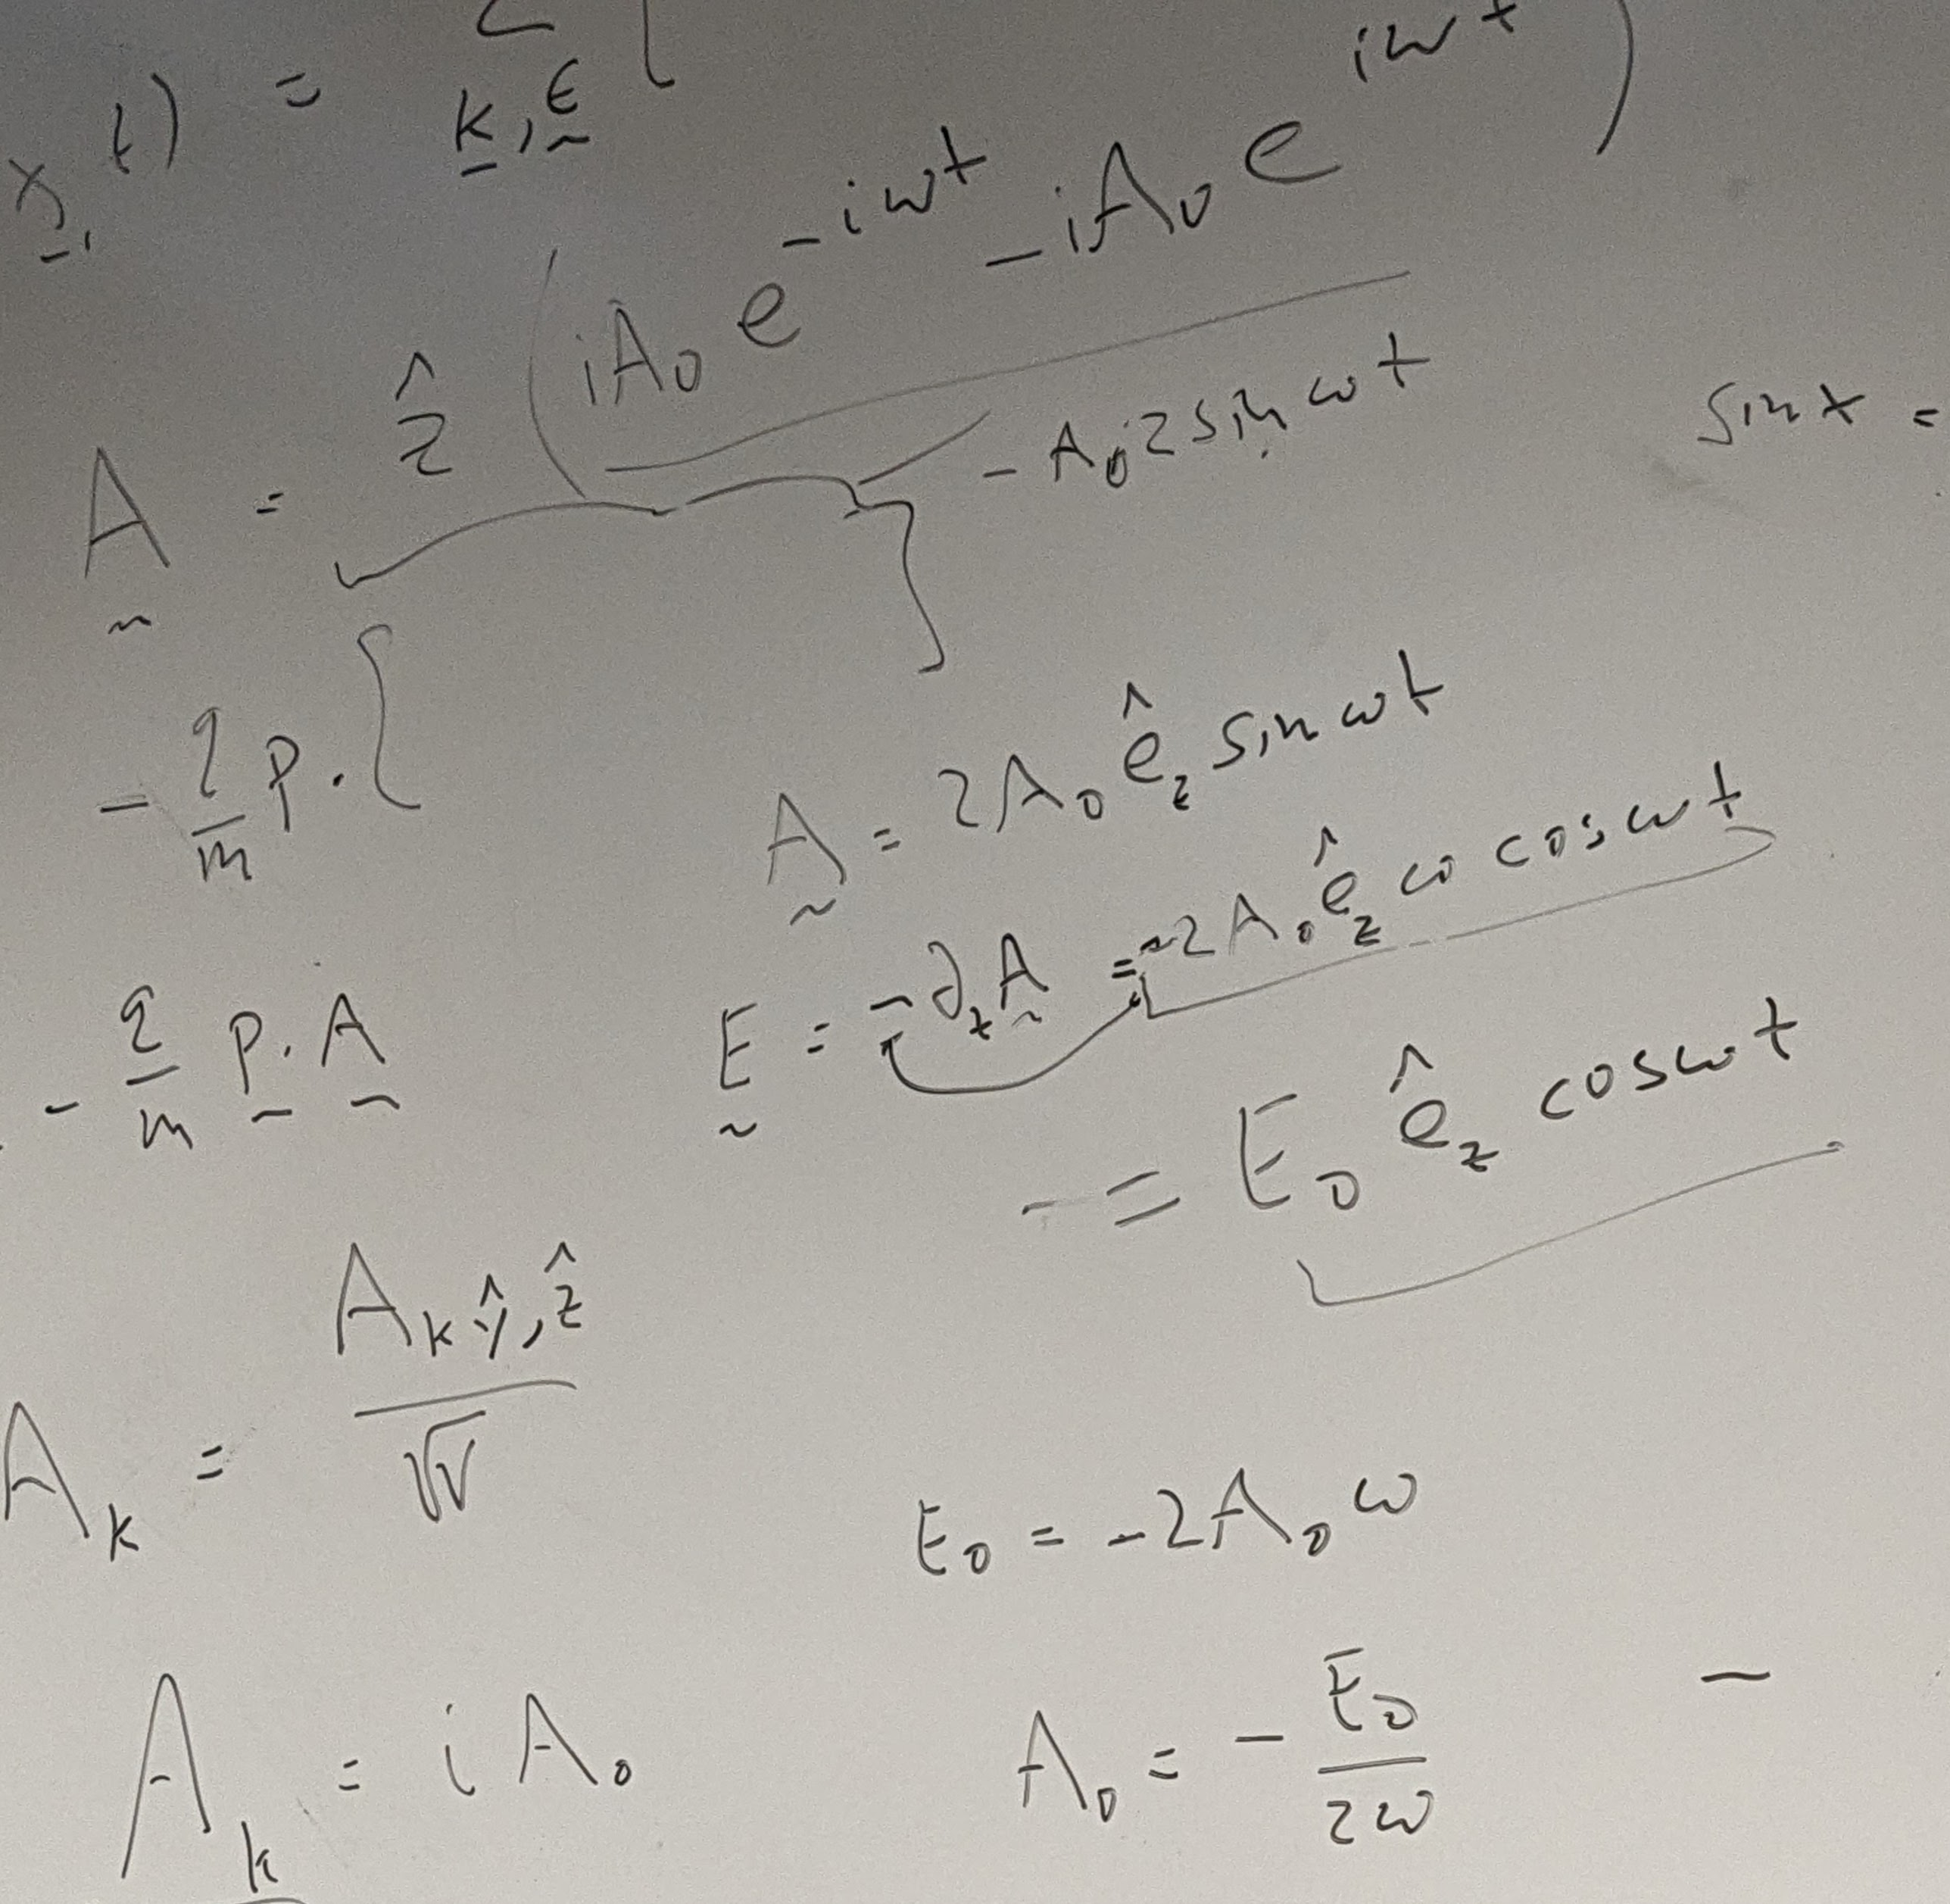
\includegraphics[width=0.8\textwidth]{PXL_20240216_204341590.jpg}
  \caption{Algebra for the dipole approximation}
\end{figure}
\end{document}